\documentclass{article}
\usepackage[utf8]{inputenc}
\usepackage{polski}
\usepackage[T1]{fontenc}
\usepackage{amsmath,amssymb,amsthm}
\usepackage{lmodern}
\usepackage{geometry}
\usepackage[dvipsnames]{xcolor}
\usepackage{hyperref}
\usepackage{array}
\usepackage{graphicx}

\newtheorem{tw}{Twierdzenie}[section]

\begin{document}

\begin{center}
    \LARGE
    \textbf{Pracownia z Analizy numerycznej (M)}

    \medskip

    Sprawozdanie do zadania {\bf P0.2}
    
    {\Large Prowadzący: Filip Chudy}

    \bigskip

    {\Large Jadwiga Świerczyńska}

    {\Large Wrocław, 28.10.2022 r.}
    
\end{center}

\bigskip


\section{Wprowadzenie}

Poniższy dokument jest rozwiązaniem zadania 2 z Pracowni 0.

\section{Tekst}

\textit{Lorem ipsum} to najczęściej stosowany tekst do demonstracji krojów pisma i kompozycji. \footnote{\url{https://pl.wikipedia.org/wiki/Lorem_ipsum}}

\subsection{Łacina}

Lorem ipsum dolor sit amet, consectetur adipiscing elit. Nulla libero orci, gravida vel est vel, commodo convallis mauris. Sed lobortis sed diam eu suscipit. Mauris tortor dolor, dictum sit amet venenatis a, ultrices quis urna. Morbi convallis lacus in massa eleifend vehicula. Mauris lacinia mi non dictum pharetra. Phasellus vel turpis tempus, sagittis odio a, dignissim nisi. Integer blandit rhoncus enim ac congue. Fusce iaculis est eget commodo tempor. Sed in odio ac turpis malesuada facilisis. Integer quis sapien eget purus dapibus vestibulum. Cras et tincidunt nisi. Lorem ipsum dolor sit amet, consectetur adipiscing elit. Nam et diam neque. Maecenas dignissim varius augue eu auctor.

Praesent consectetur magna vel diam iaculis, id pulvinar urna fermentum. Praesent iaculis diam eget felis bibendum, vitae tempor dui iaculis. Donec auctor vehicula ligula, vel tincidunt eros blandit sed. Vivamus ipsum sapien, tempor condimentum fermentum nec, volutpat vitae diam. Quisque feugiat tortor elementum scelerisque sollicitudin. Pellentesque efficitur felis et sapien vehicula vestibulum. Morbi laoreet erat at fermentum feugiat. Donec scelerisque sem at ligula malesuada, vel sollicitudin lorem pulvinar. Proin turpis nibh, porta quis quam ac, iaculis porttitor turpis.

\subsection{Wyjaśnienie}

Dlaczego przykładowy tekst, którego używa się w taki wielu miejscach na świecie, jest w języku łacińskim? Odpowiedzią prawdopodobnie jest słynna sentencja: \textit{Quidquid Latine dictum sit, altum videtur} (,,Cokolwiek powiesz po łacinie, brzmi mądrze'').

\section{Tabela}

Weźmy funkcję \(\label{fun} f(x) = x^2 + 5\). Poniższa tabela przedstawia wartości funkcji \(f\) dla kilku przykładowych argumentów.

\begin{center}
    \begin{tabular}{|c|c|}
        \hline
        \(x\) & \(f(x)\) \\
        \hline \hline
        \(-7\) & \(54\) \\
        \(-1\) & \(6\) \\
        \(0\) & \(5\) \\  
        \(2\) & \(9\) \\
        \(10\) & \(105\) \\
        \hline
    \end{tabular}
\end{center}

\section{Wykres}

W tej sekcji przedstawimy wykres funkcji \(f\) zdefiniowanej w rozdziale \ref{fun}.

\begin{figure}[h]
    \centering
    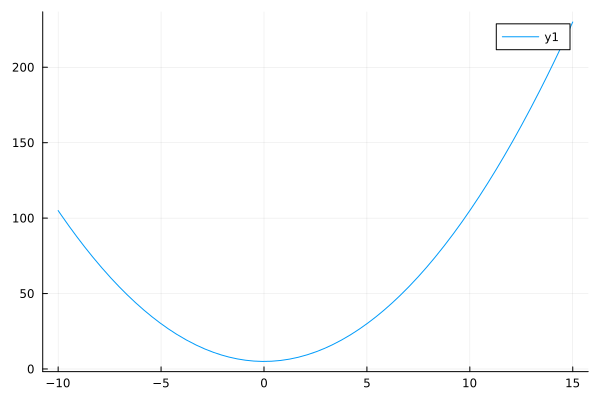
\includegraphics[width=\textwidth]{plot.png}
    \caption{Wykres funkcji \(f(x)\).}
    \label{fig:my_label}
\end{figure}

\section{Wzór -- twierdzenie Taylora}

\begin{tw}[Taylor]
    Załóżmy, że funkcja \(f : \mathbb{D} \to \mathbb{R}\)  (gdzie \(D \subseteq \mathbb{R}\)) ma pochodne wszystkich rzędów w punkcie \(x_0 \in D\). Wówczas szereg 
    \[
        \sum_{n=0}^{\infty} \frac{f^{\left(n\right)}(x_0)}{n!}(x-x_0)^n
    \]
    nazywamy szeregiem Taylora funkcji \(f\) w otoczeniu punktu \(x_0\). Szereg Taylora funkcji \(f\) w otoczeniu punktu \(x_0\) jest zbieżny do \(f(x)\) wtedy i tylko wtedy, gdy ciąg reszt \(R_n(x,x_0)\)\footnote{np. w postaci całkowej \(R_n(x,x_0) = \int\limits _{x_0}^x\frac{(x-t)^n}{n!}f^{(n+1)}(t)dt\)}
    we wzorze Taylora jest zbieżny do \(0\).
\end{tw}


\end{document}
